%#!pdfplatex
%
% How to make report01.pdf
% % latex report01.tex
% % latex report01.tex
% % dvipdf report01.dvi
% 
\documentclass{article}
\usepackage{graphicx}
\title{Programming Language Processor \\ Assignment 3}
\author{XL14608   Thiago Machado da Silva}
\date{\today}

\def\reporttrue{\let\ifreport=\iftrue}
\def\reportfalse{\let\ifreport=\iffalse}
%\reportfalse  % question
\reporttrue  % report


\begin{document}
\ifreport
\maketitle
\else
\begin{center}
{\huge Programming Language Processor Assignment 3}
\end{center}
Answer the following questions and submit your report (Word or PDF) to
tetsuya@shibaura-it.ac.jp before Jan. 19, 2015. 
The subject of your mail should be of the form ``PLP Assignment 3''.
\fi


%%%%%%%%%%%%%%%%%%%%%%%%%%%%%%%%%%%%%%%%%%%%%%%%%%%%%%%%%%%%%%%%%%%%%%%%%%%%%%%%%%%%%%%%%%%%%%%
\section*{Question 1}

To introduce the following do-while statement to PL/0', answer the following questions.
\begin{description}
 \item[Production rule] {\it statement}  $\to$ {\bf do} {\it statement} {\bf while} {\it condition}
 \item[Action] A statement '{\bf do} {\it statement} {\bf while} {\it condition}' works as follows
	    \begin{enumerate}
	     \item Execute {\it statement}.
	     \item If the value of {\it condition} is true, go to the step 1. Otherwise, exit this loop.
	    \end{enumerate}
\end{description}

\subsection*{Question 1-1}
To add a token {\tt do} to a set of starting tokens of {\it statement},
modify a function {\tt isStBeginKey} in {\tt compile.c} and explain the modification in your report.\\[0.3cm]

\ifreport
Line 253 was added, as shown in Figure~\ref{fig:q11}. Now after a "begin", a "do" can be a next token.\\
\begin{figure}[h]
  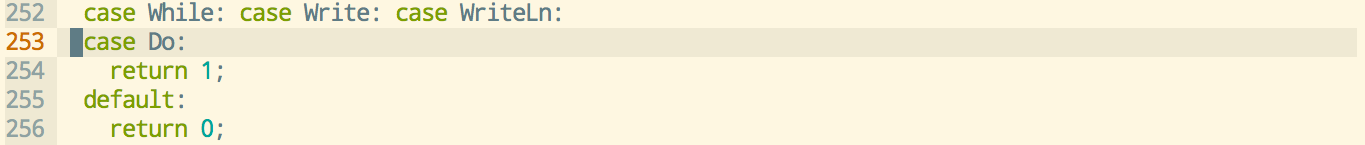
\includegraphics[scale=0.35]{./img/Q1-1.png}
  \centering
  \caption{{\tt isStBeginKey} in {\tt compile.c}.}
  \label{fig:q11}
\end{figure}
\fi
% Write your answer.



\subsection*{Question 1-2}
Modify a function {\tt statement} in {\tt compile.c} 
so that your PL/0' compiler can output object codes of Fig.\ref{fig:dowhile-code} for
do-while statements.
Explain the modification in your report.

\begin{figure}[h]
\begin{tabular}{ll}
label1: & Object codes of {\it statement} \\
        & Object codes of {\it condition} \\
        & jpc label2 \\
        & jmp label1 \\
label2: & \\
\end{tabular}
\caption{Object codes for a do-while statement}
\label{fig:dowhile-code}
\end{figure}

\ifreport
Now there is a "do" case in statement function. It was derived from the "while" case, with a few changes. The code is shown in Figure~\ref{fig:q12}. \\
\begin{figure}[h]
  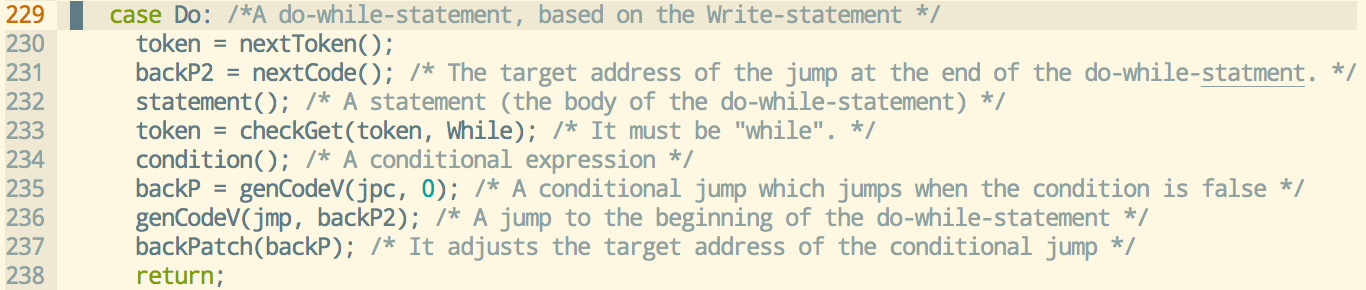
\includegraphics[scale=0.35]{./img/Q1-2.png}
  \centering
  \caption{{\tt do-while} case in {\tt statement} in {\tt compile.c}.}
  \label{fig:q12}
\end{figure}
\fi
% Write your answer.



\subsection*{Question 1-3}
What does your PL/0' compiler outputs when your PL/0' compiler compiles
and executes a PL/0' program do.pl0 of Fig. \ref{fig:do-while}?

\begin{figure}[h]
\begin{verbatim}
var x;
begin
   x := 0;
   do begin
      write x;
      writeln;
      x := x + 1
   end
   while x < 3
end.
\end{verbatim}
\caption{A test program {\tt do.pl0}}\label{fig:do-while}
\end{figure}

\ifreport
The output is shown in Figure~\ref{fig:q13}. The left side is the output itself, and the right side is the pl0 code (I decided to show the code again). \\
\begin{figure}[h]
  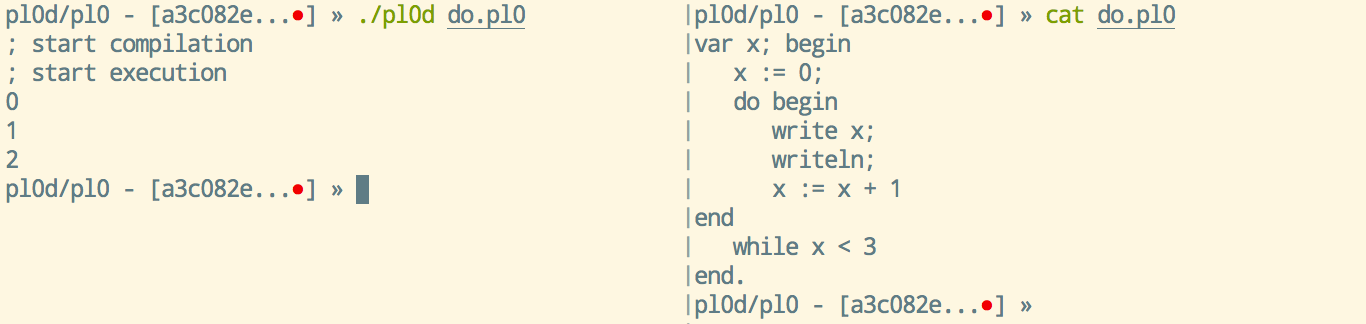
\includegraphics[scale=0.35]{./img/Q1-3.png}
  \centering
  \caption{output from {\tt do.pl0}.}
  \label{fig:q13}
\end{figure}
\fi
% Write your answer.




%%%%%%%%%%%%%%%%%%%%%%%%%%%%%%%%%%%%%%%%%%%%%%%%%%%%%%%%%%%%%%%%%%%%%%%%%%%%%%%%%%%%%%%%%%%%%%%
\newpage
\section*{Question 2}
Answer the following questions to add the following repeat-until statement to PL/0'.

\begin{description}
 \item[Production rule] {\it statement}  $\to$ {\bf repeat} {\it statement} {\bf until} {\it condition}
 \item[Action] A statement '{\bf repeat} {\it statement} {\bf until} {\it condition}' works as follows.
	    \begin{enumerate}
	     \item Execute {\it statement}.
	     \item If the value of {\it condition} is false, go to the step 1. Otherwise, exit this loop.
	    \end{enumerate}
\end{description}

\subsection*{Question 2-1}
Write object codes for the repeat-until statement 
like object codes for the do-while statement of Fig.\ref{fig:dowhile-code}.\\[0.3cm]


\ifreport
\begin{figure}[h]
\begin{tabular}{ll}
label1: & Object codes of {\it statement} \\
        & Object codes of {\it condition} \\
        & jpc label1 \\
\end{tabular}
\caption{Object codes for a repeat-until statement.}
\label{fig:q21}
\end{figure}
\fi



\subsection*{Question 2-2}
Modify {\tt getSource.h} and {\tt getSource.c} to register two tokens
{\tt repeat} and {\tt until} to your PL/0' compiler.
Explain the modification in your report.\\[0.3cm]


\ifreport
The modification is shown in Figure~\ref{fig:q22}. The left side is the {\tt getSource.h} and the right side is the {\tt getSource.c}. In the {\tt .h} file the change is in line 15 in the "keys" enum, and in the {\tt .c} file the changes are in lines 47 and 48 in "KeyWdT" vector. Those are needed so they can be valid tokens when reading the code.\\
\begin{figure}[h]
  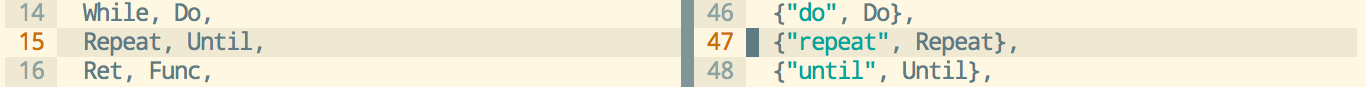
\includegraphics[scale=0.35]{./img/Q2-2.png}
  \centering
  \caption{{\tt getSource.h} (left side) and {\tt getSource.c} (right side).}
  \label{fig:q22}
\end{figure}
\fi




\subsection*{Question 2-3}
To add a token {\tt repeat} to a set of starting tokens of {\it statement},
modify a function {\tt isStBeginKey} in {\tt compile.c} and explain the modification in you report.\\[0.3cm]


\ifreport
Line 253 was modified, as shown in Figure~\ref{fig:q23}. The same reason from Question 1-1 apply here.
\begin{figure}[h]
  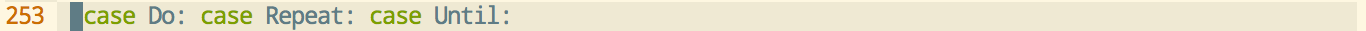
\includegraphics[scale=0.35]{./img/Q2-3.png}
  \centering
  \caption{{\tt isStBeginKey} in {\tt compile.c}.}
  \label{fig:q23}
\end{figure}
\fi
% Write your answer.


\subsection*{Question 2-4}
Modify a function {\tt statement} in {\tt compile.c}
so that your PL/0' compiler can output object codes for repeat-until statements.
Explain the modificaiton in your report.


\ifreport
It's similar to the while or do-while from Question 1-2. Basically, the code executes a statement, and jump to the begginning if the codition is false. The code is shown in Figure~\ref{fig:q24}. \\
\begin{figure}[h]
  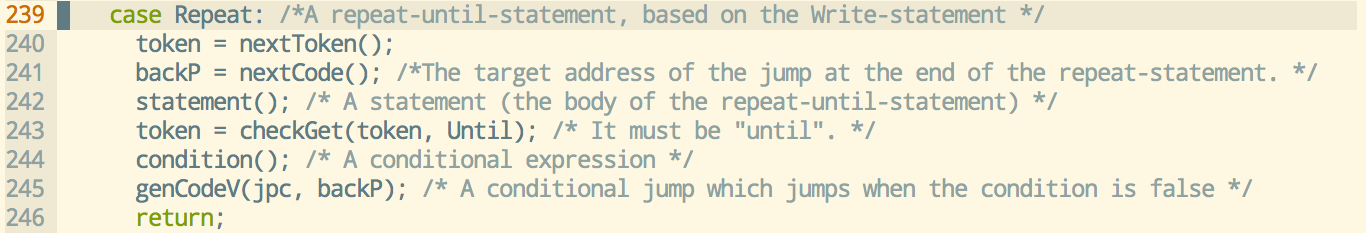
\includegraphics[scale=0.35]{./img/Q2-4.png}
  \centering
  \caption{{\tt repeat-until} case in {\tt statement} in {\tt compile.c}.}
  \label{fig:q24}
\end{figure}
\fi
% Write your answer.


\subsection*{Question 2-5}
What does your PL/0' compiler outputs when your PL/0' compiler compiles
and executes a PL/0' program {\tt repeat.pl0} of Fig.\ref{fig:repeat-until}?

\begin{figure}[h]
\begin{verbatim}
var x;
begin
   x := 0;
   repeat begin
      write x; 
      writeln;
      x := x + 1
   end
   until x=3
end.
\end{verbatim}
\caption{A test program {\tt repeat.pl0}}\label{fig:repeat-until}
\end{figure}


\ifreport
The output is shown in Figure~\ref{fig:q25}. The left side is the output itself, and the right side is the pl0 code. \\
\begin{figure}[h]
  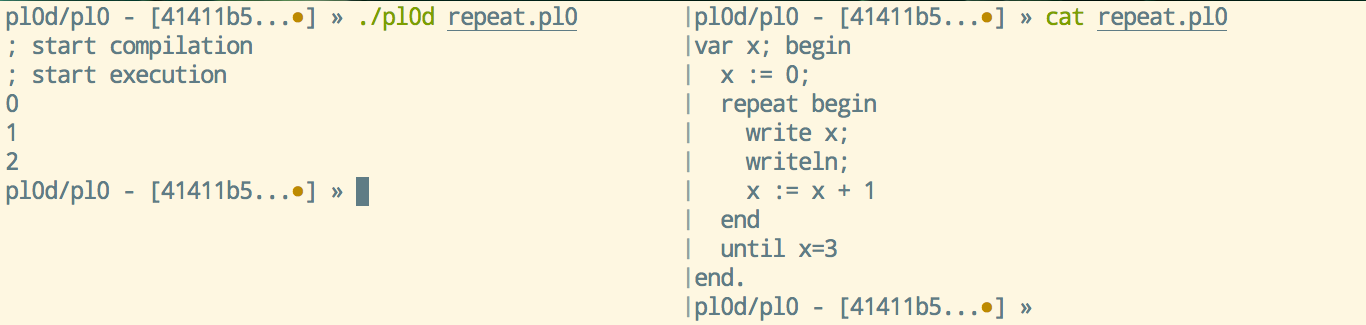
\includegraphics[scale=0.35]{./img/Q2-5.png}
  \centering
  \caption{output from {\tt do.pl0}.}
  \label{fig:q25}
\end{figure}
\fi
% Write your answer.


%%%%%%%%%%%%%%%%%%%%%%%%%%%%%%%%%%%%%%%%%%%%%%%%%%%%%%%%%%%%%%%%%%%%%%%%%%%%%%%%%%%%%%%%%%%%%%%
\newpage
\section*{Question 3}
Answer the following questions to add the following if-then-else statement to PL/0'.

\begin{description}
 \item[Production rule] {\it statement}  $\to$ {\bf if} {\it condition} {\bf then} 
       ${\it statement}_1$ ({\bf else} ${\it statement}_2$ $\vert$ {$\epsilon$})
 \item[Action] A statement '{\bf if} {\it condition} {\bf then} 
	    ${\it statement}_1$ ({\bf else} ${\it statement}_2$ $\vert$ {$\epsilon$})'
	    works as follows.
	    \begin{enumerate}
	     \item Evaluate {\it condition}.
	     \item If the value of {\it condition} is true, execute ${\it statement}_1$.
	     \item If the value of {\it condition} is false and ${\it statement}_2$ exists, 
		   execute ${\it statement}_2$.
	    \end{enumerate}
 \item[Description] To resolve ambiguity of the grammar of PL/0', 
	    we use the following rule.
	    \begin{itemize}
	     \item When we find an {\bf else}, we relate the {\bf else} to the nearest {\bf then}
		   which has not be related to any {\bf else} yet.
	    \end{itemize}
\end{description}


\subsection*{Question 3-1}
Write object codes for 
a statement '{\bf if} {\it condition} {\bf then}
${\it statement}_1$ {\bf else} ${\it statement}_2$'
like object codes for a do-while statement of Fig.\ref{fig:dowhile-code}.


\ifreport
\begin{figure}[h]
\begin{tabular}{ll}
        & Object codes of {\it condition} \\
        & jpc label1 \\
        & Object codes of {\it statement1} \\
        & jmp label2 \\
label1: & If "else": Object codes of {\it statement2} \\
label2: & \\
\end{tabular}
\caption{Object codes for a if-else statement.}
\label{fig:q31}
\end{figure}
\fi


\subsection*{Question 3-2}
Modify {\tt getSource.h} and {\tt getSource.c} to register a token
{\tt else} to your PL/0' compiler.
Explain the modification in your report.\\[0.3cm]


\ifreport
The modification is shown in Figure~\ref{fig:q32}, just like Question 2-2. The left side is the {\tt getSource.h} and the right side is the {\tt getSource.c}. In the {\tt .h} file the change is in line 13 in the "keys" enum, and in the {\tt .c} file the changes are in lines 45 in "KeyWdT" vector. Those are needed so it can be a valid token when reading the code.\\
\begin{figure}[h]
  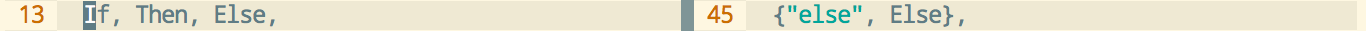
\includegraphics[scale=0.35]{./img/Q3-2.png}
  \centering
  \caption{{\tt getSource.h} (left side) and {\tt getSource.c} (right side).}
  \label{fig:q32}
\end{figure}
\fi


\subsection*{Question 3-3}
Modify a function {\tt statement} in {\tt compile.c}
so that your PL/0' compiler can output object codes for if-then-else statements.
Explain the modificaiton in your report.\\[0.3cm]


\ifreport
It's a modification from the original "if" case. After the execution of the statement1, the execution should jump to the end of the case. Before that, if the condition evaluation is false, the execution should jump to the statement2, if there is a "else" token. The code is shown in Figure~\ref{fig:q33}. \\
\begin{figure}[h]
  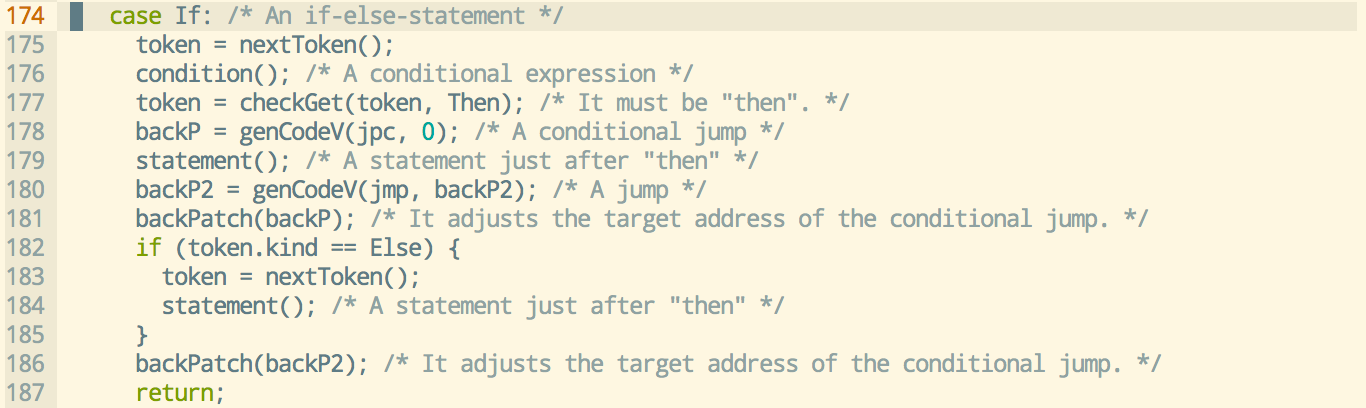
\includegraphics[scale=0.35]{./img/Q3-3.png}
  \centering
  \caption{{\tt if-then-else} case in {\tt statement} in {\tt compile.c}.}
  \label{fig:q33}
\end{figure}
\fi
% Write your answer.


\subsection*{Question 3-4}
What does your PL/0' compiler outputs when your PL/0' compiler compiles
and executes a PL/0' program else.pl0 of Fig.\ref{fig:if-then-else}?

\begin{figure}[h]
\begin{verbatim}
var x;
begin
   x := 0;
   while x<3 do begin
      if x < 1 then write 0
      else if x < 2 then write 1
      else write 2;
      writeln;
      x := x+1;
   end;
end.
\end{verbatim}
\caption{A test program else.pl0}\label{fig:if-then-else}
\end{figure}


\ifreport
The output is shown in Figure~\ref{fig:q34}. The left side is the output itself, and the right side is the pl0 code. \\
\begin{figure}[h]
  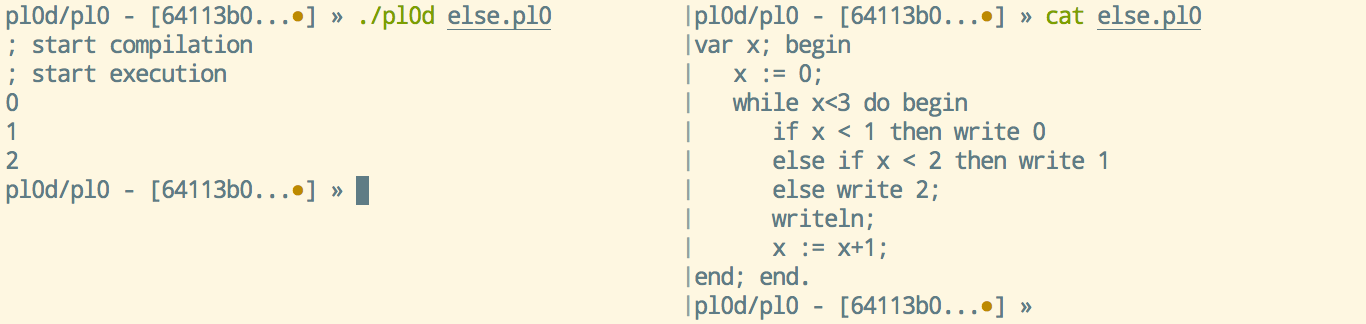
\includegraphics[scale=0.35]{./img/Q3-4.png}
  \centering
  \caption{output from {\tt do.pl0}.}
  \label{fig:q34}
\end{figure}
\fi
% Write your answer.


%%%%%%%%%%%%%%%%%%%%%%%%%%%%%%%%%%%%%%%%%%%%%%%%%%%%%%%%%%%%%%%%%%%%%%%%%%%%%%%%%%%%%%%%%%%%%%%
\newpage
\section*{Question 4}
Answer the following questions to introduce one-dimensional array to PL/0'.


\subsection*{Question 4-1}
Explain how to modify the grammar of PL/0' to introduce one-dimensional array to PL/0'.\\[0.3cm]

\ifreport
The grammar needs to identify the brackets when declaring variables or when acessing variables values, when this variable is an array. In array declaration, inside the brackets there is a constant number referrering to the length of this array. In array access, inside the brackets there is an expression that evaluates to a number, the array index.\\[0.3cm]
\fi
% Write your answer.

\subsection*{Question 4-2}
Do you need new instructions to the PL/0' virtual machine for one-dimensional array?
If you need new instructions, define thier mnemonics and their actions.\\[0.3cm]


\ifreport
Yes, two instructions: "ldr" and "str". ldr refers to "relative load", and str to "relative store". \\
ldr pushes to the top of the stack some value residing in another position in the same stack. This position is evaluated using the array "base position" (this information is with the ldr instruction) and the "index" (this information should be at the top of the stack).\\
str is similar to ldr: changes the value from some position in the stack. The new value comes from the top of the stack, and the "index" comes right below it. The "index" is relative to the array "base position" (information contained in the str instruction).\\
In the stack, the array position works as follows: The base position is referred by the array name (in the nameTable). Every increment in the "index" decrements the "absolute position" in the stack. Also the first (zero index) position is not at the same position as the array base, but it's position minus one.\\[0.3cm]
\fi
% Write your answer.


\subsection*{Question 4-3}
Modify your PL/0' compiler so that it can support one-dimensional array.
Explain the modification in your report.\\[0.3cm]

\ifreport
To register the new instructions the {\tt codegen.h} (line 5 in {\tt codes enum}) and {\tt codegen.c} (lines 113 and 115 in {\tt updateRef} for flagging, 139 and 141 in {\tt printCode} for printing, 201 to 203 and 206 to 209 in {\tt execute} for the actions) files were changed, as shown in Figures~\ref{fig:q431} and~\ref{fig:q432}.\\

\begin{figure}[h]
  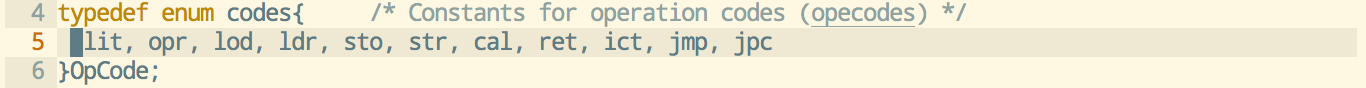
\includegraphics[scale=0.35]{./img/Q4-3-1.png}
  \centering
  \caption{{\tt codegen.h}.}
  \label{fig:q431}
\end{figure}

\begin{figure}[h]
  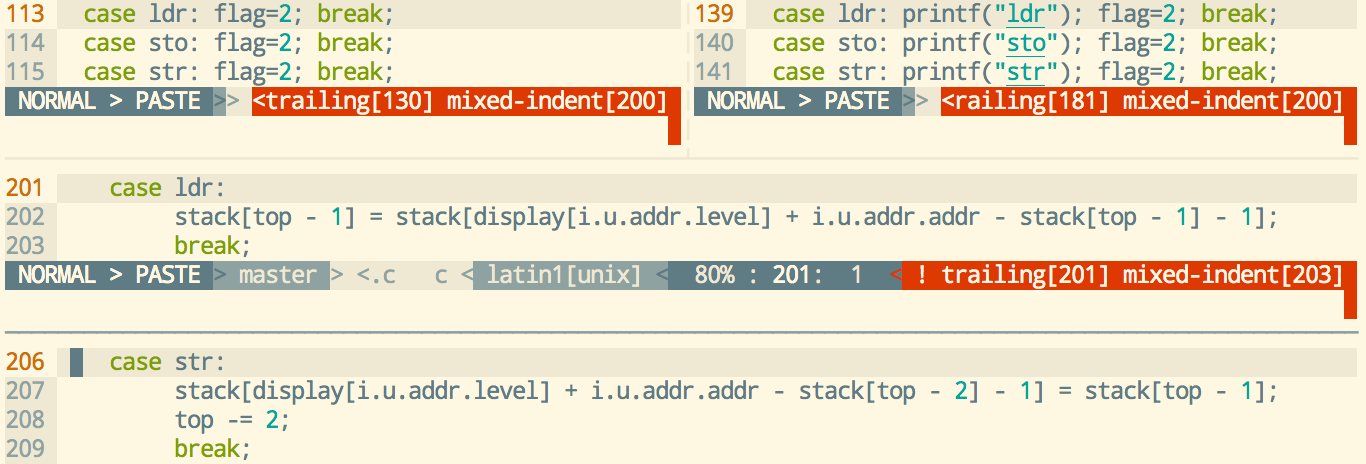
\includegraphics[scale=0.35]{./img/Q4-3-2.png}
  \centering
  \caption{{\tt codegen.c}.}
  \label{fig:q432}
\end{figure}

To register the brackets as valid tokens, there is changes in the {\tt getSource.c} (lines 65 and 66 in {\tt KeyWdT array} and line 108 in {\tt initCharClassT}) and in the {\tt getSource.h} (line 23), as shown in the Figure~\ref{fig:q433}.\\

\begin{figure}[h]
  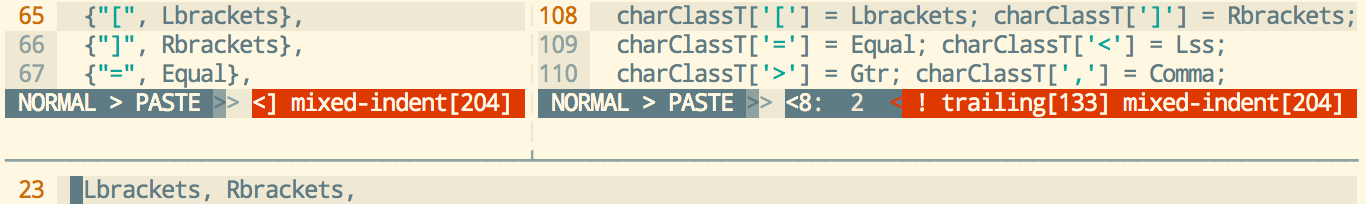
\includegraphics[scale=0.35]{./img/Q4-3-3.png}
  \centering
  \caption{{\tt getSource.c} (upper side) and {\tt getSource.h} (down side).}
  \label{fig:q433}
\end{figure}

To register arrId (array kind of identifier), {\tt table.h} (line 5) and {\tt table.c} (line 42) files are modified. Also in {\tt table.c} the {\tt enterTarr} function is created (lines 125 to 139), it creates a new array identifier and reserves space in the stack according to the array length. Both files are shown in Figure~\ref{fig:q434}.\\

\begin{figure}[h]
  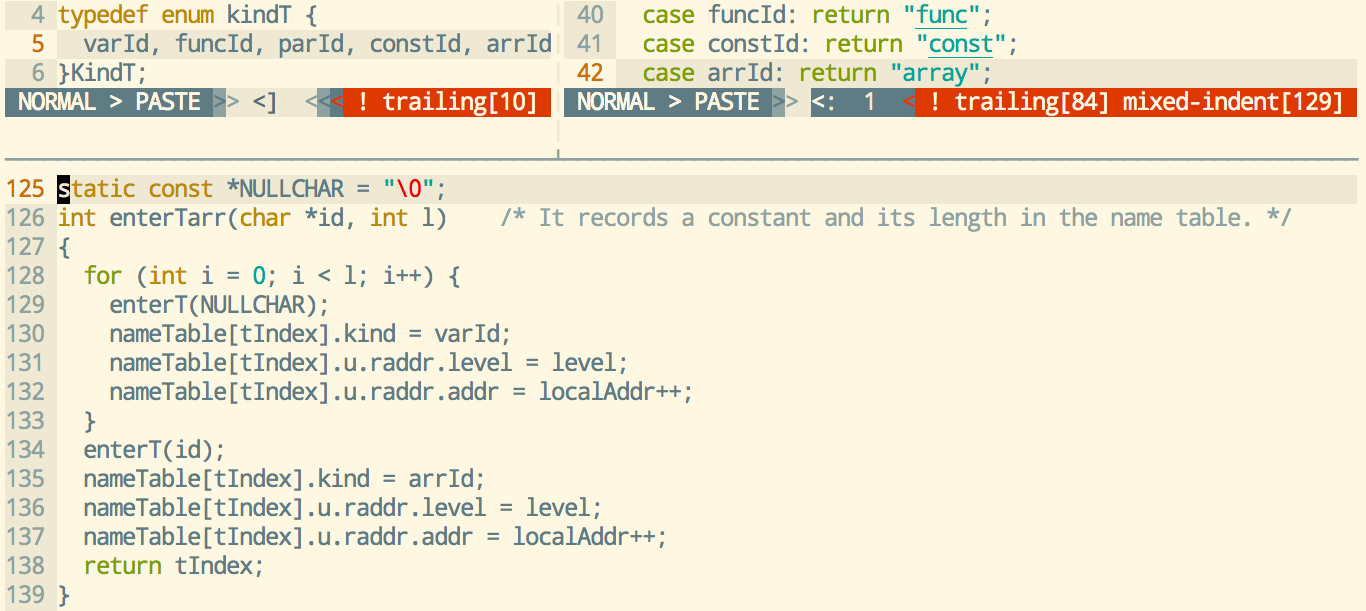
\includegraphics[scale=0.35]{./img/Q4-3-4.png}
  \centering
  \caption{{\tt table.h} (upper-left side) and {\tt table.c} (upper-right and down side).}
  \label{fig:q434}
\end{figure}

The {\tt compile.c} file is also modified. There is a modification in {\tt varDecl} function (when {\tt token.kind} equals {\tt Id}, lines 102 to 118, to declare a new array). This is for the array declaration, and a constant number is required between the brackets. See Figure~\ref{fig:q435}.\\

\begin{figure}[h]
  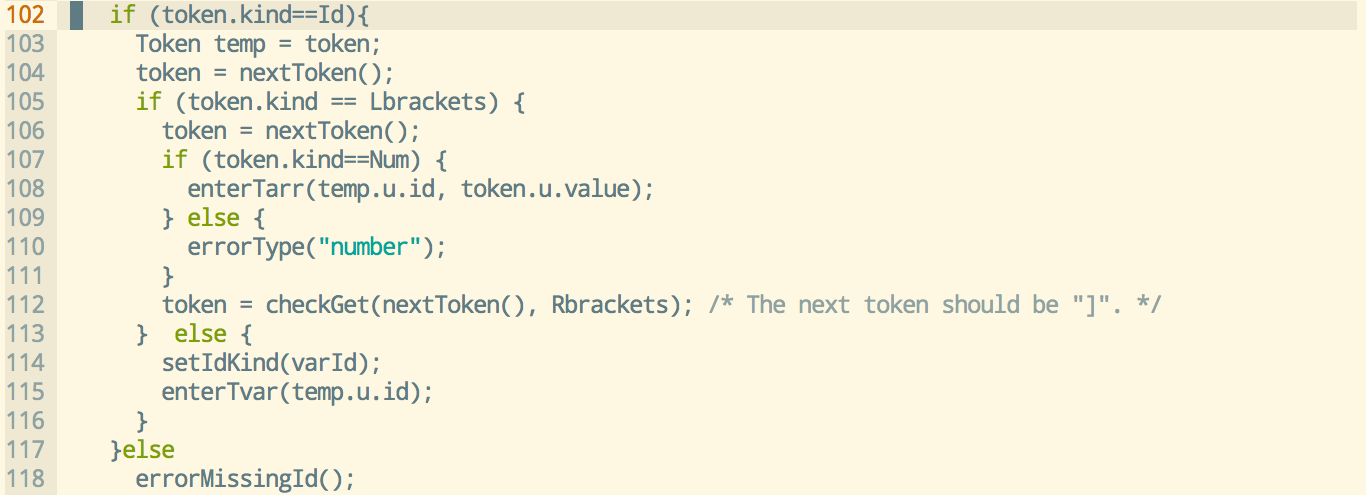
\includegraphics[scale=0.35]{./img/Q4-3-5.png}
  \centering
  \caption{{\tt varDecl} in {\tt compile.c}.}
  \label{fig:q435}
\end{figure}

The next change is in {\tt statement} function (in {\tt case Id}, lines 176 to 192). This is for array access and it supports an expression between the brackets. See Figure~\ref{fig:q436}.\\

\begin{figure}[h]
  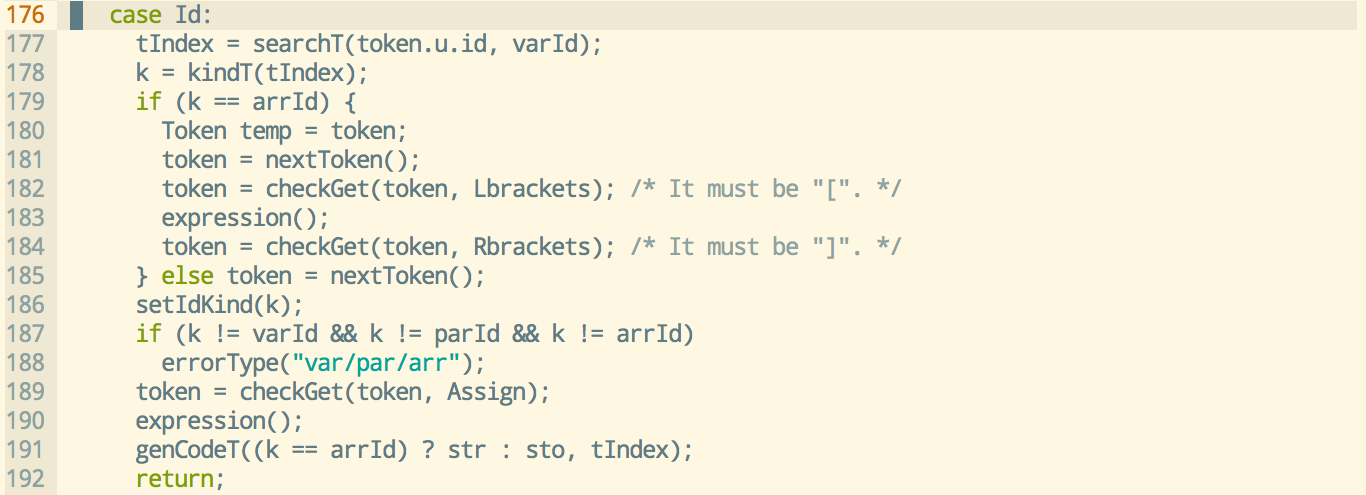
\includegraphics[scale=0.35]{./img/Q4-3-6.png}
  \centering
  \caption{{\tt statement} in {\tt compile.c}.}
  \label{fig:q436}
\end{figure}

The last one is in {\tt factor } function (added {\tt case arrId}, lines 368 to 374). This is also for array access, and an expression is supported between the brackets. See Figure~\ref{fig:q437}.\\

\begin{figure}[h]
  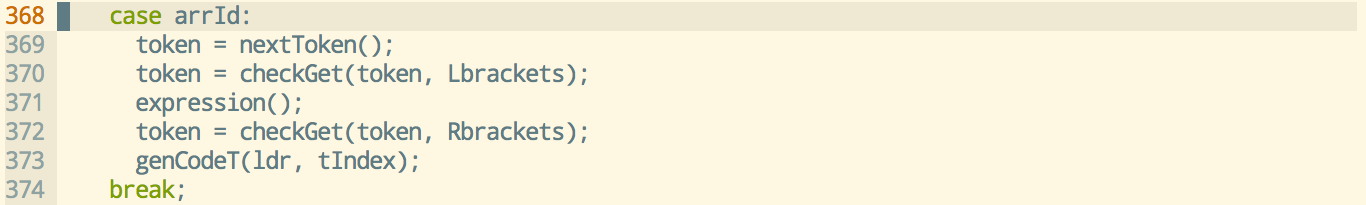
\includegraphics[scale=0.35]{./img/Q4-3-7.png}
  \centering
  \caption{{\tt factor} in {\tt compile.c}.}
  \label{fig:q437}
\end{figure}
\clearpage
\fi
% Write your answer.

\subsection*{Question 4-4}
Write a simple test program {\tt array.pl0} for one-dimensional array.
Explain the test program and what your PL/0' compiler outputs when it
compiles and executes the test program.


\ifreport
The output is shown in Figure~\ref{fig:q44}. The left side is the output itself, and the right side is the pl0 code.\\
Line 1: the array is created, it's length equals 2. \\
Line 2: the variable's first index value is changed (statement's code).\\
Line 4: the variable's first index value is printed (factor's code).\\
\begin{figure}[h]
  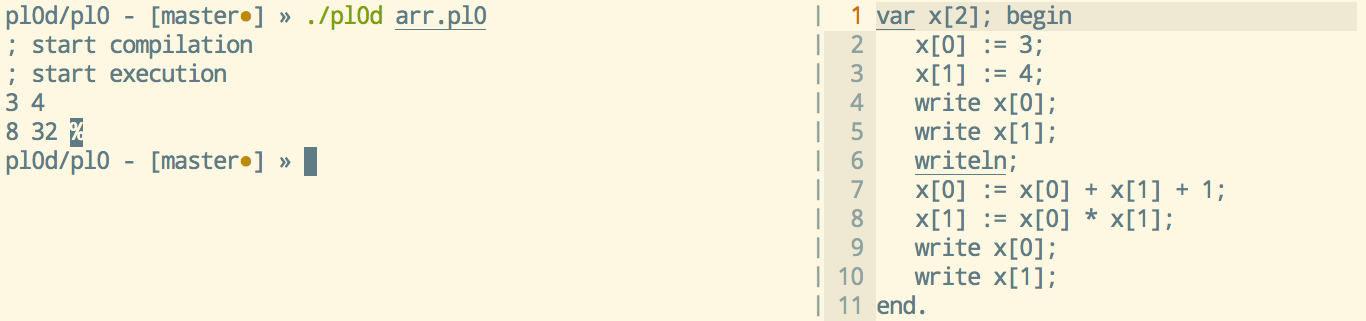
\includegraphics[scale=0.35]{./img/Q4-4.png}
  \centering
  \caption{output from {\tt do.pl0}.}
  \label{fig:q44}
\end{figure}
\fi
% Write your answer.


%%%%%%%%%%%%%%%%%%%%%%%%%%%%%%%%%%%%%%%%%%%%%%%%%%%%%%%%%%%%%%%%%%%%%%%%%%%%%%%%%%%%%%%%%%%%%%%
\newpage
\section*{Question 5}
Answer the following questions to introduce procedures (functions withaout any return values) to PL/0'.

We use the following statement to call a procedure with $n$ arguments.
\begin{quote}
 {\bf call} {\it procedure}($arg_1$, $arg_2$, $\dots$, $arg_n$)
\end{quote}


\subsection*{Question 5-1}
Explain how to modify the grammar of PL/0' to introduce procedures to PL/0'.

\subsection*{Question 5-2}
Do you need new instructions to the PL/0' virtual machine for procedures?
If you need new instructions, define thier mnemonics and their actions. 


\subsection*{Question 5-3}
Modify your PL/0' compiler so that it can support procedures.
Explain the modification in your report.

\ifreport
(Answer)\\
\fi
% Write your answer.


\subsection*{Question 5-4}
Write a simple test program {\tt proc.pl0} for procedures.
Explain the test program and what your PL/0' compiler outputs when it
compiles and executes the test program.


\ifreport
(Answer)\\
\fi
% Write your answer.



%%%%%%%%%%%%%%%%%%%%%%%%%%%%%%%%%%%%%%%%%%%%%%%%%%%%%%%%%%%%%%%%%%%%%%%%%%%%%%%%%%%%%%%%%%%%%%%
\newpage
\section*{Question 6}
Introduce your own idea to your PL/0' compiler.

\ifreport
(Answer)\\
\fi
% Write your answer.



%%%%%%%%%%%%%%%%%%%%%%%%%%%%%%%%%%%%%%%%%%%%%%%%%%%%%%%%%%%%%%%%%%%%%%%%%%%%%%%%%%%%%%%%%%%%%%%
%\vspace{1cm}
\ifreport
\else
\section*{How to submit your report}
Submit an archive file which includes the following files to
tetsuya@shibaura-it.ac.jp before Jan. 19, 2015.
\begin{enumerate}
 \item Your report file report03.pdf or report03.doc (Word)
 \item All source files of your PL/0' compiler
 \item Makefile
 \item The following test programs
       \begin{enumerate}
	\item array.pl0
	\item proc.pl0
	\item test programs for your own idea
       \end{enumerate}
\end{enumerate}

The subject of your mail should be of the form ``PLP Assignment 3''.

A name of the archive file should be of the form ``your\_id.tgz'' like ``xa14000.tgz''.
You can make the the archive file on Linux as follows.
\begin{enumerate}
 \item Create a directory whose name is your ID.
       For example, create a directory ``xa14000'' as follows if your ID is ``xa14000''.
       \begin{quote}
	{\tt \% mkdir} {\tt xa14000} 
       \end{quote}

 \item Copy all files into the directory.
 \item Make your archive file using tar command as follows.
       \begin{quote}
	{\tt \% tar zcvf} \ \ {\tt xa14000}{\tt .tgz} \ \ {\tt xa14000}
       \end{quote}
\end{enumerate}

Check your archive file before submission. You can expand your archive
file as follows.
\begin{quote}
 {\tt \% tar zxvf} \ \ {\tt xa14000}{\tt .tgz}
\end{quote}


\fi

\end{document}
